\vspace{-0pt}
\section{Evaluation and Analysis} \label{sec:evaluation}
\vspace{-5pt}
%
In addition to the real chip evaluation, we also want to investigate the impact of design parameters in REMARK.
To explore larger design space, we develop a simulator, \emph{NVnodeSim} to gain more insights in designing TPC system.
In this section, we first present the simulator in Sec.~\ref{sec:expSettings}. 
Then, we tune the simulator to different settings and evaluate it with more general benchmarks to show how different design options affect the system performance in Sec.~\ref{sec:expEvaluation} and ~\ref{sec:expParaAnalysis}. 
Based on the observations, we summarize three design rules in Sec~\ref{sec:expRules}. 

%\vspace{-5pt} 
\subsection{Experiment Settings} \label{sec:expSettings}
\vspace{-5pt}
% Simulator
The inputs of NVnodeSim are power traces and benchmark profiles.
The power traces are solar power data from an open source database~\cite{midc2015solar}.
The benchmarks consist of three kinds of operations as shown in Table~\ref{tab:benchmarks}.
All parameters are extracted from datasheets or the cycle-accurate processor simulator Keil C.
Three common computing tasks for IoT are adopted.
Two I/O interfaces and five peripherals are also used, including sensors, transceivers, and an off-chip memory.
%We construct sensor node benchmarks by combining different computation operations, I/O interface and peripherals.

\begin{table}[t]
\begin{center}
    \vspace{-5pt}
\caption{Benchmarks: compute, I/O and peri. oper.}  \label{tab:benchmarks}
    \vspace{-5pt}
\Fsize{8}
\renewcommand{\arraystretch}{1.5}

% Computing Operations Table
%\begin{tabular*}{9cm}{@{\extracolsep{\fill}}Ic|cIc|cIc|cI}
\begin{tabular}{Im{1.15cm}<{\centering}|m{0.85cm}<{\centering}Im{1.15cm}<{\centering}|m{0.8cm}<{\centering}Im{1.15cm}<{\centering}|m{0.85cm}<{\centering}I}
    \Xhline{1.2pt}
    compute operation       & time /cycles          & compute operation      & time /cycles          & compute operation       & time /cycles           \\
    \Xhline{1.2pt}
    crc16                & $122$                   & rsa                   & $409$       & fft16                  & $275$                  \\
    \Xhline{1.2pt}
\end{tabular}

% I/O Operations Table
%\begin{tabular*}{9cm}{@{\extracolsep{\fill}}Ic|c|c|cI}
\begin{tabular}{Im{1.4cm}<{\centering}|c|c|m{1.9cm}<{\centering}I}
    \Xhline{1.2pt}
    I/O bus             & init time/cycles          & read time/cycles               & write time/cycles            \\
    \Xhline{1.2pt}
    I2C                 & $403$                         & $270 + 90 \times N$        & $180 + 90 \times N\tnote{*}$        \\
    \Xhline{1pt}
    SPI                 & $171$                         & $320 + 80 \times N$         & $320 + 80 \times N$        \\
    \Xhline{1.2pt}
\end{tabular}

% Peripherals Table
%\begin{tabular*}{9cm}{@{\extracolsep{\fill}}Ic|c|c|c|cI}
\begin{tabular}{Ic|c|c|c|cI}
    \Xhline{1.2pt}
    Peripheral                  & Chip                  & init./ms          & I/O bus       & exec time/ms    \\
    \Xhline{1.2pt}
    ZigBee                       & ML7266             & 531        & SPI        & $5.7 + 0.14 \times N$    \\
    %\Xhline{1pt}
    %Bluetooth                  & CC2540              & 1101        & SPI       & $1.2 + 0.37 \times N$    \\
    %\Xhline{1pt}
    %Light Sensor              & NOA1305          & 1451        & I2C       & 0.644    \\
    \Xhline{1pt}
    Acc. Sensor           & LIS331DLH       & 2391        & I2C       & 0.451    \\
    \Xhline{1pt}
    Image Sensor             & LUPA1300        & 14,952     & I2C       & 118.0    \\
    \Xhline{1pt}
    Tmp. Sensor               & TMP101           & 566          & I2C       & 0.283    \\
    \Xhline{1pt}
    FeRAM Mem            & FM25V20          &  76           & SPI        & --    \\
    \Xhline{1.2pt}
\end{tabular}

%\begin{tablenotes}
%    \footnotesize
%    \item[*] The number of transmited bytes.
%\end{tablenotes}

    \vspace{-10pt}
\end{center}
%\end{threeparttable}
\end{table} 

%
To validate the accuracy of NVnodeSim, Table~\ref{tab:SimValidateResults} compares the task execution time between NVnode and NVnodeSim.
It shows that NVnodeSim provides reasonable accuracy for architecture-level exploration.

\begin{table}[t]
\begin{center}
\vspace{-10pt}
\caption{Accuracy evaluation of NVnodeSim.} \label{tab:SimValidateResults}
\vspace{-5pt}
\Fsize{8}
\renewcommand{\arraystretch}{1.5}
%\setlength{\tabcolsep}{1pt}
\begin{tabular}{Im{1.37cm}<{\centering}Ic|m{0.89cm}Ic|m{0.99cm}IcI}
    \Xhline{1.2pt}
    \multirow{2}{*}{Benchmarks}     & \multicolumn{2}{cI}{Failure Times}       & \multicolumn{3}{cI}{Execution Time/ms} \\
                                                            \Xcline{2-6}{1pt}
                                                            & NVnode               & Sim                             & NVnode                & Sim                      & Error         \\
    \Xhline{1pt}
    RSA                                                & 3                           & 3                                 & 3.560                    & 3.512                   & -1.35\%        \\
    \Xhline{1pt}
    CRC                                                & 1                          & 1                                 & 1.316                    & 1.309                   & -0.53\%        \\
    \Xhline{1pt}
    MemLS                                           & 12                        & 11                               & 12.05                    & 11.99                   & -0.49\%        \\
    \Xhline{1pt}
    Sense                                               & 42                        & 42                               & 42.95                    & 42.38                   & -1.33\%        \\
    \Xhline{1.2pt}
\end{tabular}
\end{center}
    \vspace{-10pt}
\end{table} 

%\vspace{-5pt}
\subsection{Evaluation with Multiple Benchmarks} \label{sec:expEvaluation}
\vspace{-5pt}
% 
We further evaluate the performance of REMARK with ten additional benchmarks on the simulator.
Fig.~\ref{fig:I/OPerformance} (a) shows the recovery overhead distribution under ten benchmarks.
On average, REMARK reduces total overhead by 64\% compared with SDRB.
Fig.~\ref{fig:I/OPerformance} (b) shows that, the overhead of SDRB rises rapidly when multiple peripherals are included in the program.
This is because the re-initialization overhead grows rapidly.
The system even falls into deadlock when the re-initialization overhead is too large to complete during power failure intervals.
Thanks to the efficient \emph{`init-used'} strategy, the re-initialization overhead of REMARK stays modest.
From the experiment, we can see that \emph{REMARK can recover the system with multiple peripherals more efficiently and reliably}.

%
\begin{figure*}[t]
    \centering
    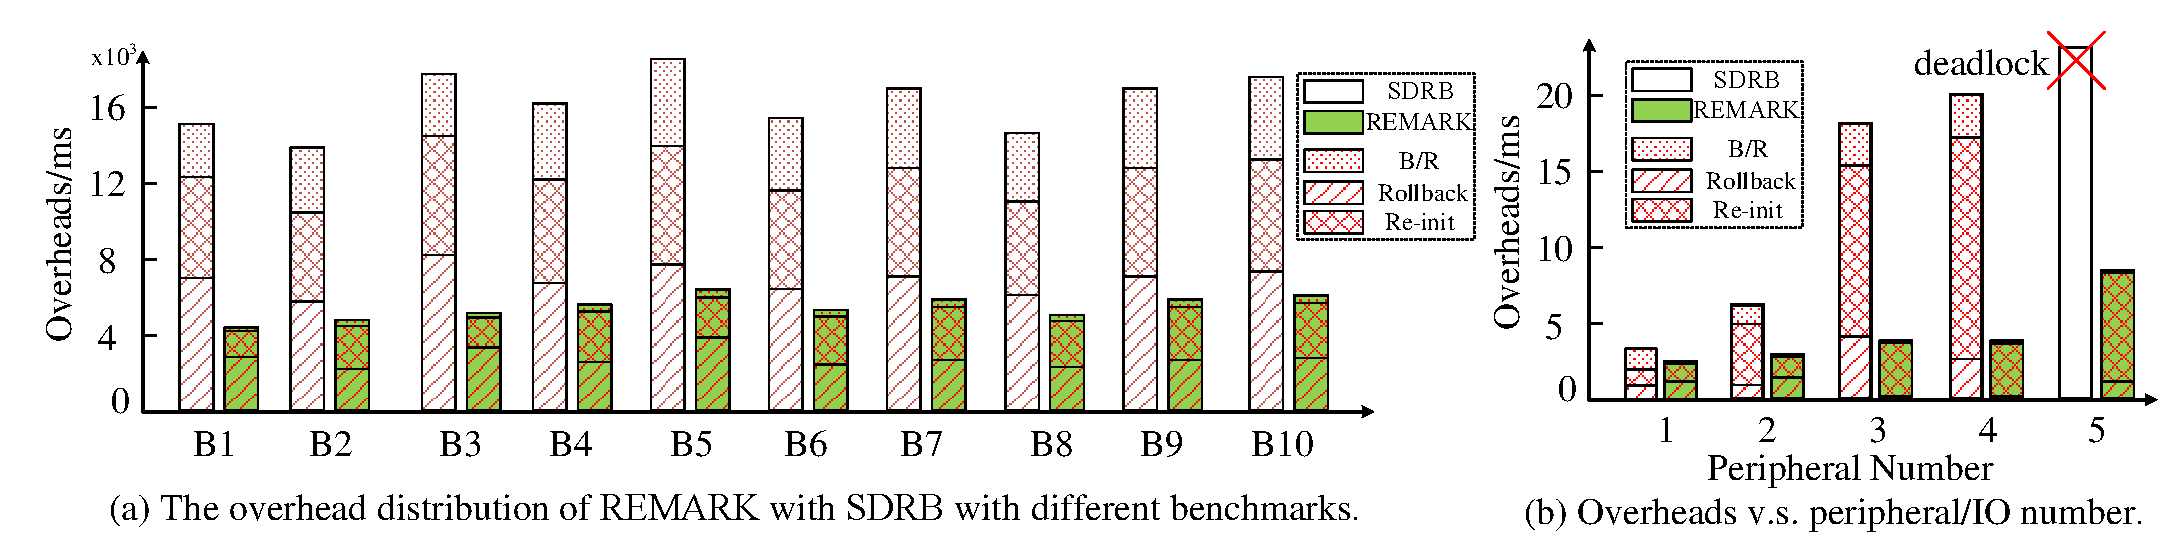
\includegraphics[width=0.9\textwidth]{Fig16_ExpIOPerformance.pdf}
    \vspace{-5pt}
    \caption{Recover overheads comparison between REMARK and SDRB.}
    \vspace{-0pt}
    \label{fig:I/OPerformance}
\end{figure*}

%\vspace{-5pt}
\subsection{Analysis the Peripheral Related Factors} \label{sec:expParaAnalysis}
\vspace{-5pt}
%
An important observation in Fig.~\ref{fig:I/OPerformance} is that the re-initialization and rollback overheads dominate the recovery overhead of REMARK.
These overheads are caused by peripheral disruptions.
The operation distribution in the program profile has a direct effect on peripheral disruptions.
Therefore, we explore the impact of three distribution factors of I/O and peripheral operations as below to gain insights on TPC system design.

%
\begin{figure}[t]
    \centering
    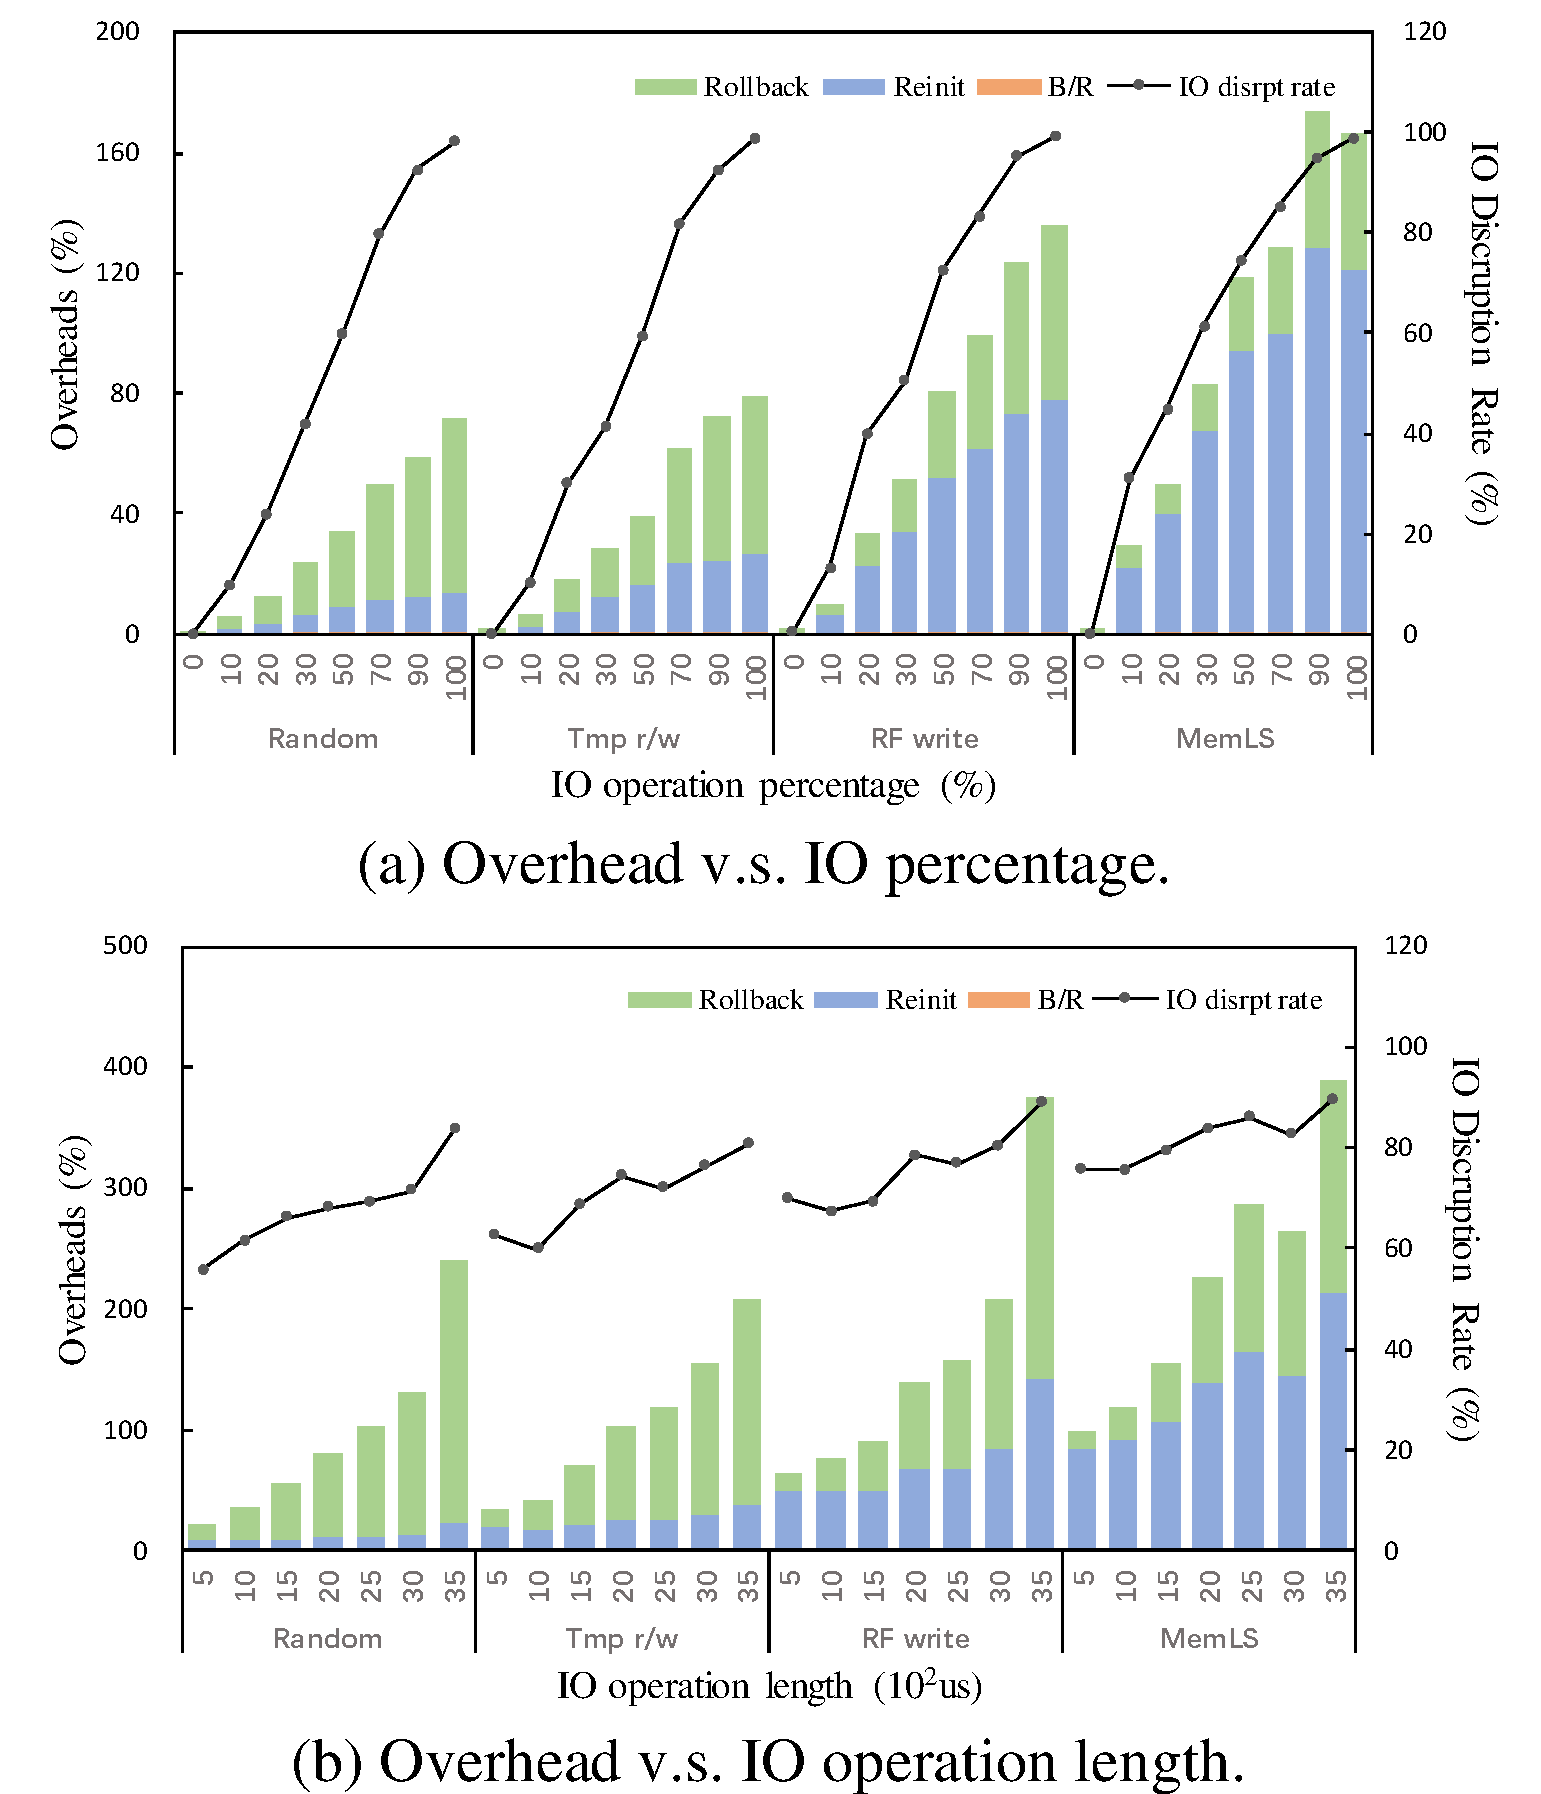
\includegraphics[width=0.4\textwidth]{Fig15_ExpPeriOperDistribute.pdf}
    \vspace{-5pt}
    \caption{{The performance overheads with various peripheral operation percentage and length.}}
    \vspace{-5pt}
    \label{fig:ExpPeriOperDistribute}
\end{figure}

\vspace{5pt}
\noindent\textbf{Peripheral Operation Percentage.} \\
Fig.~\ref{fig:ExpPeriOperDistribute} (a) shows the overheads and the failure times using benchmarks containing different peripheral operation percentages.
When more peripheral operations are used in a benchmark, power failures are more likely to cause peripheral disruptions.
According to the results, when the percentage increases, the total overhead increases slower than linear trend.
The reason is that recovering peripherals introduces more peripheral operations which increase its actual percentage compared with the original program.
Therefore, when a benchmark contains more than $70\%$ peripheral operations, the actual percentage approaches saturation and the total overhead grows slowly.

\vspace{5pt}
\noindent\textbf{Peripheral Operation Length.} \\
The length of each I/O operation affects the rollback distance during recovery.
Fig.~\ref{fig:ExpPeriOperDistribute} (b) shows the effect of lengths on the peripheral disruption times and the recovery overheads.
Rollback overhead increases when the length of peripheral operation increases from $0.5ms$ to $3.5ms$.
This is because longer peripheral operations may cause higher rollback distance.
Therefore, \emph{shorten the length of each peripheral operation can reduce the overhead of single recovery}.

\begin{comment}
% length v.s. the disruption times
Fig.~\ref{fig:ExpPeriOperDistribute} (b) shows that more peripheral disruptions take place when the length grows.
In statistics analysis, the peripheral disruption rate is affected only by peripheral operation percentage.
However, longer peripheral recover procedure increases this percentage, causes significant avalanche effects and leads to higher peripheral disruption rate.
In conclusion, \emph{the longer I/O operation length also increases the I/O disruption probability because of the avalanche effect}.
\end{comment}

\vspace{5pt}
\noindent\textbf{Overlap of I/O and Peripheral Operations.} \\
%
Since the processor and peripherals operate in parallel, the interaction among these devices also affects the performance of REMARK.
This part explores the impact of the overlap between I/O and peripheral operations.

In a wireless sensor node, I/O operations are executed by the processor, including off-chip memory accesses, sensor configurations, etc.
Peripheral operations are executed on peripherals, including sensing and data transmission tasks.
In such a system, the total recovery overhead of the system is determined by the largest overhead either on the processor or the peripheral.
Table~\ref{tab:OverheadPeriTask} shows the recovery overhead under different overlap ratios, where I/O/Peri. overlap is the overlap percentage of the I/O and peripheral operations.
The I/O/Peri. overlap ranges from $0$ to $100\%$ in two different benchmarks (sensing and data transmission). 
The breakdown of the recovery overhead of processor and peripherals are shown.
The stall time represent that the processor waits for the peripherals.
Overhead reduction shows how much reduction is achieved when there are more overlaps compared with the program with no overlap.
Results show that, the overhead decreases as much as $36.5\%$ when the overlap percentage increases.

Since most of sensor nodes work in a periodical way, overlapping I/O operations of previous loops with peripheral operations in current loop could be an effective solution to avoid large recovery overhead.
Therefore, \emph{with REMARK, software designer should overlap I/O and peripheral operations as much as possible to reduce the stall time of recovery process}.

\begin{table}[t]
\begin{center}
    \vspace{-5pt}
\caption{Overheads with different overlap percentages.} \label{tab:OverheadPeriTask}
    \vspace{-5pt}
\Fsize{8}
\renewcommand{\arraystretch}{1.5}
\begin{tabular}{Im{2.1cm}Ic|c|cIc|c|cI}%33.8 %40.3
    \Xhline{1.2pt}
    Benchmarks                                    & \multicolumn{3}{cI}{Sensing}                  & \multicolumn{3}{cI}{Data Transmission} \\
    \Xhline{1pt}
    I/O/Peri. overlap                               & 0\%           & 50\%         & 100\%             & 0\%           & 50\%         & 100\%        \\
    \Xhline{1pt}
    proc. overhead /\%                          & 44.9           & 43.6           & 43.4                & 43.4          & 42.7          & 41.7        \\
    \Xhline{1pt}
    peri. overhead /\%                           & 18.4            & 16.0           & 18.3                & 80.9          & 74.8          & 74.2       \\
    \Xhline{1pt}
    stall time/\%                               & 18.4            & 10.8           & 6.1                  & 80.9          & 62.4          & 39.2       \\
    \Xhline{1pt}
    Total overhead /\%                         & 63.3           & 54.4           & 49.5                & 124.3        & 105.1         & 78.9       \\
    \Xhline{1pt}
    {Overhead Reduction/\%}                         & --           & {14.0}           & {21.8}               & --        & {15.4}         & {36.5}       \\
    \Xhline{1.2pt}
\end{tabular}
\end{center}
\vspace{-10pt}
\end{table} 

\subsection{Analysis Conclusion} \label{sec:expRules}
\vspace{-5pt}
%
The evaluation experiments show that REMARK is able to support the reliability and task progress of a TPC system with multiple peripherals.
According to these analysis, we summarize three design rules for performance-aware software:

\begin{itemize}
    \item \textbf{Smaller I/O percentage.} 
        Reduce I/O operations as much as possible in TPCs to avoid expensive recovery overhead.
 
    \item \textbf{Shorter I/O operation length.}  
        Shorter I/O operations have smaller overhead. It is benefit to split a long I/O operation into several shorter ones.
     
    \item \textbf{More overlap between I/O and peripheral operations.} 
        Overlapping parallel operations can remove the stall time of the recovery process. It is also benefit to overlap the sensing and transmission operations in different cycles.

\end{itemize}










